
%LET'S GO TEAM!!! ONE LESS SECTION
%We are unstoppppable --> DAB DAB DAB

In this part of the Attachment the method to compute optimum constellation configuration given some requirements will be discussed. The method applied is based in some conditions that must be fulfilled to asses that global coverage is obtained.

The variables that this method take as inputs have been enumerated in the report. they can also be found in the table~\ref{t:varRange}

\subsubsection{Global Coverage Conditions}


\textbf{Same plane condition}\

In order to fulfill the desired coverage, the distance between two satellites on the same plane must not be more than two times the central angle $\beta$. This condition is visually represented in Figure~\ref{fig:ConditionGCoverage} .\\

\textbf{Different plane condition}\

To accomplish the coverage requirements, the distance between two satellites on different planes must not be more than the central anglep $\beta$. This condition is visually represented in Figure~\ref{fig:ConditionGCoverage} .\\

\begin{figure}[H] %[b] % h / H / b / t
	\centering
	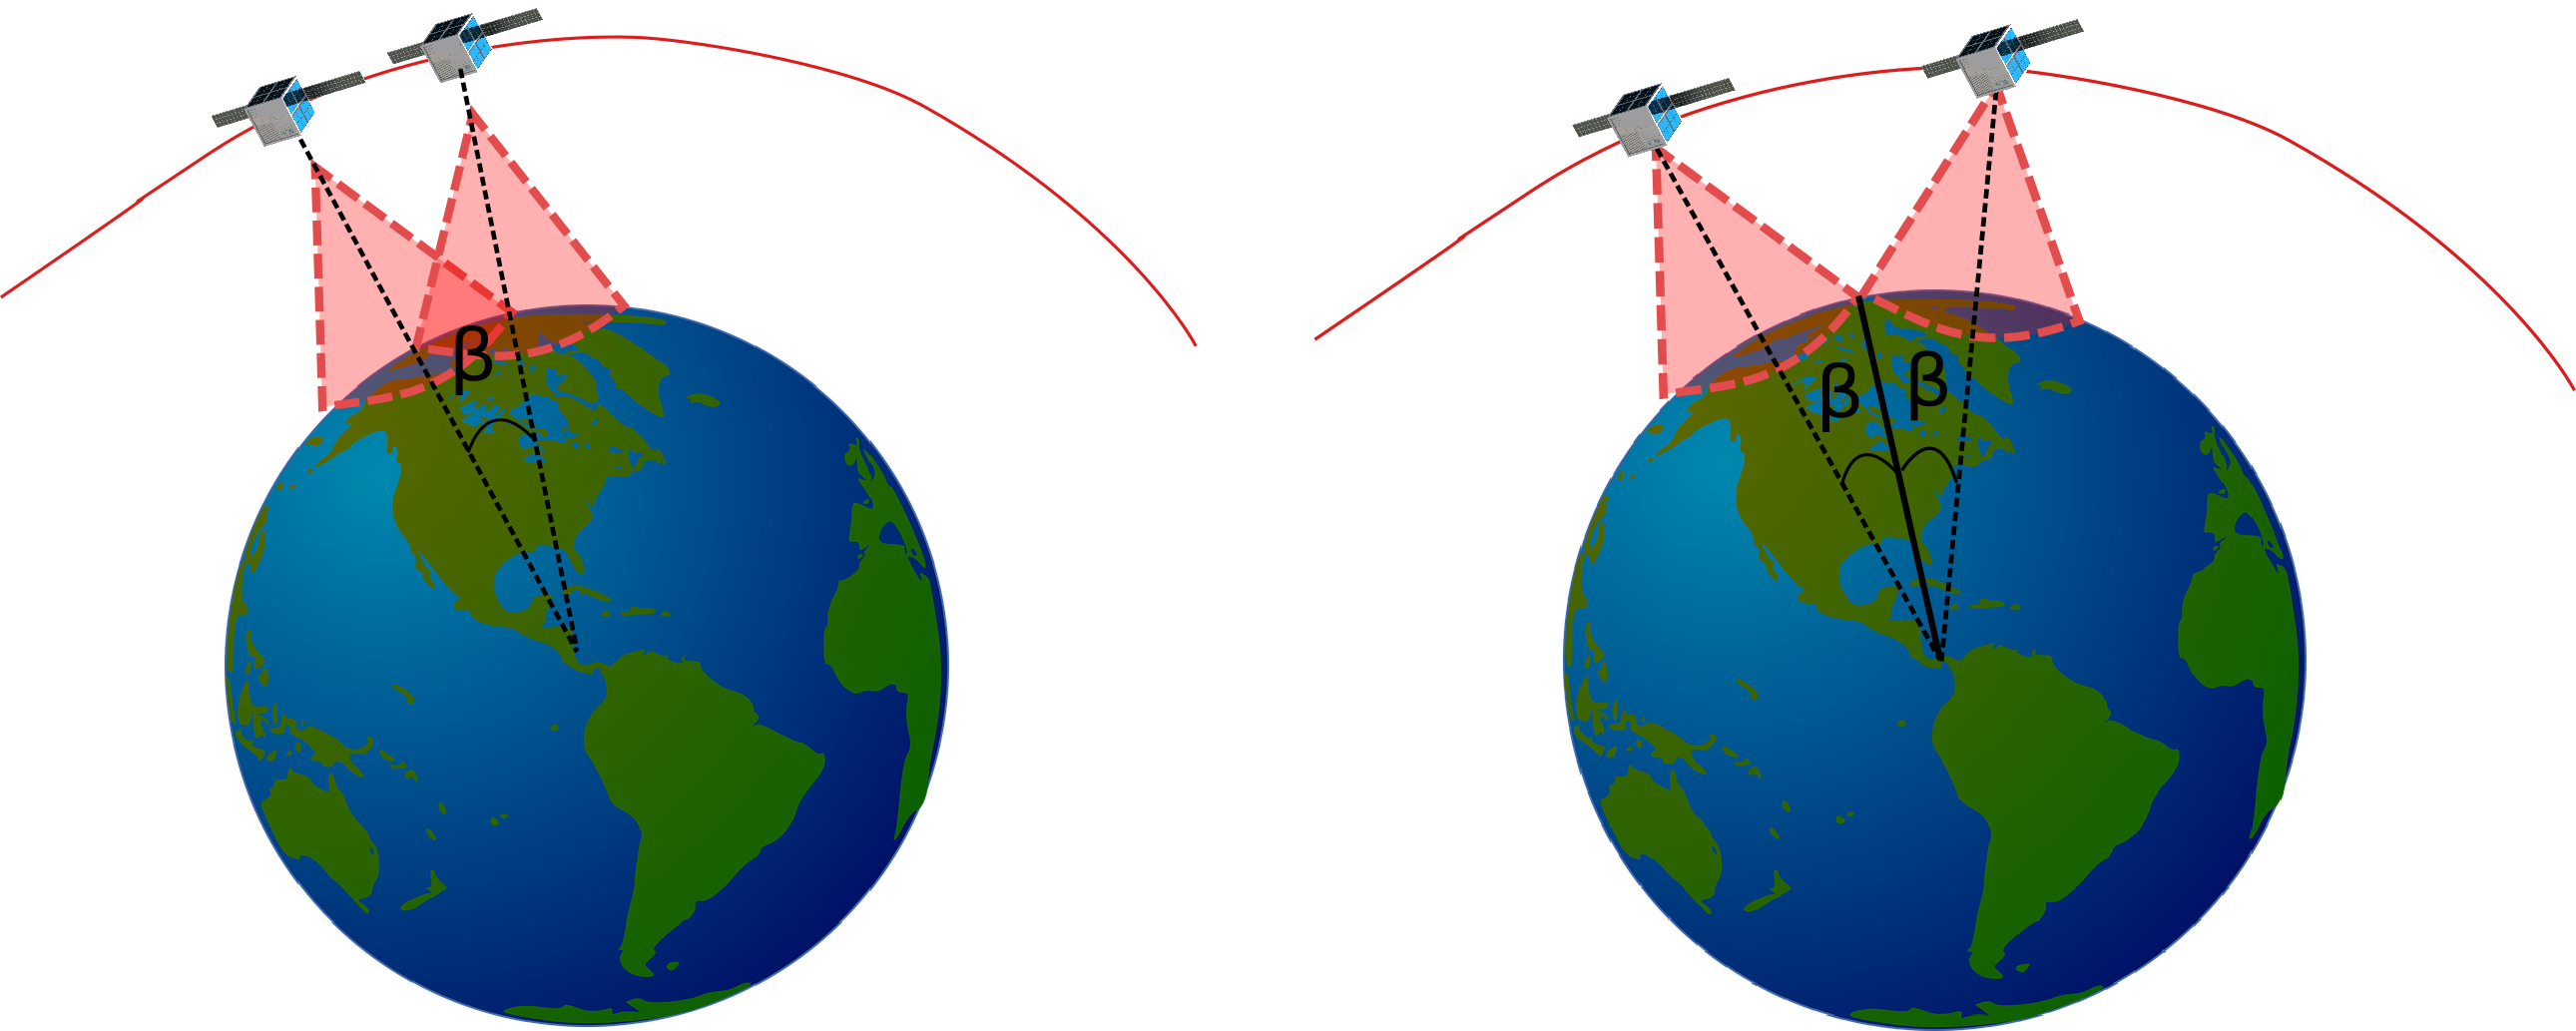
\includegraphics[width=.8\textwidth]{./testing/ConditionGCoverage.png}\\
	\caption{Geometrical conditions needed to fulfill global coverage.\\
			On the left: Condition between satellites of different planes.\\
			On the right: Condition between satellites of the same plane}
	\label{fig:ConditionGCoverage}
\end{figure}

\subsubsection{Procedure of Testing Method}

A MATLAB routine has been designed to compute the described algorithm. This routine can be found in the ANNEX VI 1.4. In this phase different values of all the variables have been computed in order to found the most suitable solution. The values tested are the following:

\begin{table}[H]
\centering
\begin{tabular}{|c|l|}
\hline
\multicolumn{2}{|c|}{Coverage Testing Method Variables}     \\ \hline
$$typeC$$          & {[}180 210 225 240 360{]} {[}º{]} 			 \\ \hline
$\varepsilon$      & {[}20{]} {[}º{]}                         \\ \hline
$$h$$              & {[}540-550{]} {[}km{]}                   \\ \hline
$$in$$             & {[}70-80{]} {[}º{]}                 \\ \hline
$n_{p}$            & {[}5-12{]}                        \\ \hline
$N_{pp}$           & {[}10-24{]}                    \\ \hline
\end{tabular}
\caption{Testing Values for the Coverage Testing Method}
\label{t:varRange}
\end{table}  

\textbf{General Solution}\\

The program has been run for all the range specified above in order to find the best constellations options. As it can be deduced, both the number of planes and satellites decreases when increasing height because as explained before the footprint of the satellites gets incremented with height.
If height is left as a constant, a less intuitive results are obtained. We have now different configurations in terms of number of satellites an planes due to the variation of the inclination angle of the planes.
In the Figure~\ref{fig:graph120} the results obtained for one of the analysed configurations are shown. \\

\begin{figure}[H] %[b] % h / H / b / t
	\centering
	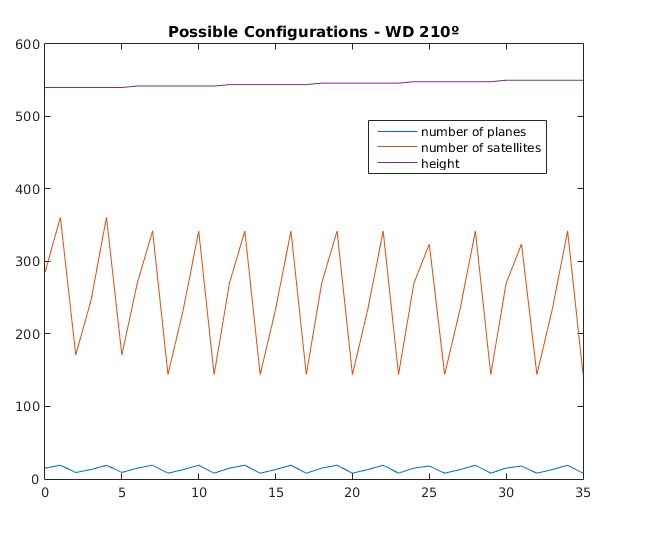
\includegraphics[width=.5\textwidth]{./testing/graph210.png}\\
	\caption{Possible satellite configurations for a 210º Walker Delta configuration}
	\label{fig:graph120}
\end{figure}

As mentioned in the Report, once the results have been obtained, three of them have been plotted to visually verify if the coverage obtained is the desired. Below this paragraph the ground track and a conceptual view of the earth can be seen for these three configurations.

\begin{figure}[H] %[b] % h / H / b / t
	\centering
	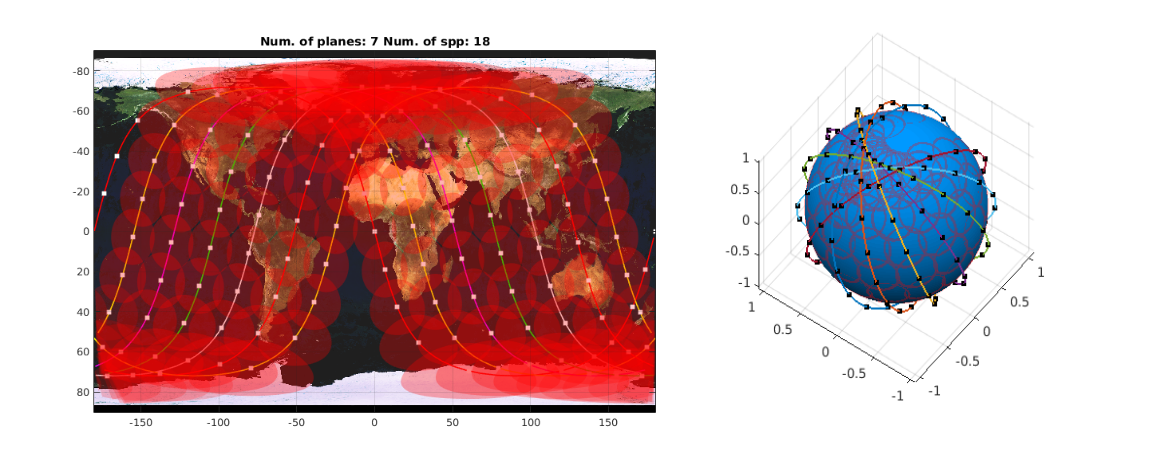
\includegraphics[width=1\textwidth]{./testing/WB180.png}\\
	\caption{Ground track and spherical representation for a 180º Walker Delta configuration}
	\label{fig:graph120}
\end{figure}

\begin{figure}[H] %[b] % h / H / b / t
	\centering
	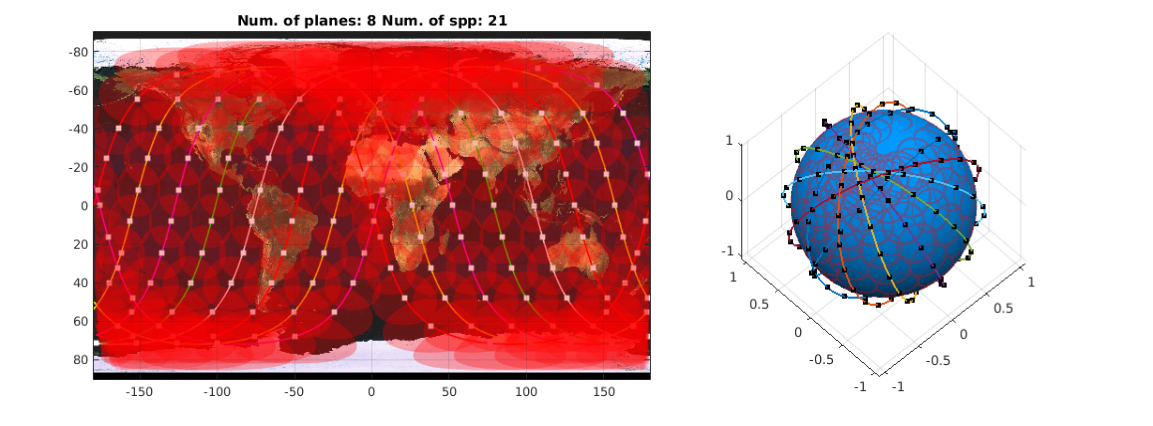
\includegraphics[width=1\textwidth]{./testing/WB210.png}\\
	\caption{Ground track and spherical representation for a 210º Walker Delta configuration}
	\label{fig:graph120}
\end{figure}

\begin{figure}[H] %[b] % h / H / b / t
	\centering
	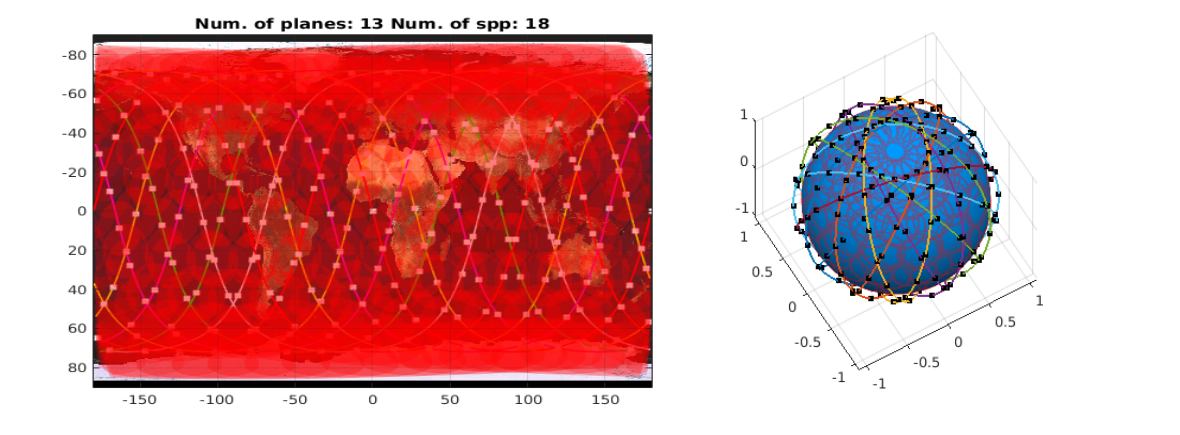
\includegraphics[width=1\textwidth]{./testing/WB360.png}\\
	\caption{Ground track and spherical representation for a 360º Walker Delta configuration}
	\label{fig:graph120}
\end{figure}

To realize these graphs has been necessary to develop a some codes that, again, can be found in the ANNEX VI, in the section 1.6.